\documentclass[11pt]{article}

\usepackage[margin=1in]{geometry}
\usepackage{amsmath,amssymb,amsthm,mathtools,bm}
\usepackage{booktabs,array}
\usepackage{siunitx}
\usepackage{pgfplots}
\usepackage{algorithm}
\usepackage{algpseudocode}
\usepackage{csquotes}
\usepackage{microtype}
\usepackage{hyperref}
\usepackage[capitalise,noabbrev]{cleveref}
\pgfplotsset{compat=1.18}
\hypersetup{colorlinks=true,linkcolor=black,citecolor=black,urlcolor=blue!50!black}

\theoremstyle{plain}
\newtheorem{proposition}{Proposition}[section]
\theoremstyle{definition}
\newtheorem{definition}[proposition]{Definition}

\newcommand{\R}{\mathbb{R}}
\newcommand{\code}[1]{\texttt{#1}}
\newcommand{\relu}{\operatorname{ReLU}}
\newcommand{\softmax}{\operatorname{softmax}}
\newcommand{\abs}[1]{\left\lvert #1 \right\rvert}

\title{Axon: A Single-Binary Engine for Small Tabular,\\Image and Text Models, with a Second-Order Tree Booster}
\author{Ryan Wetzstein}
\date{November 2026 \quad (describes v0.11.0)}

\begin{document}
\maketitle

\begin{abstract}
Axon is a single Rust binary that trains small models for the Nexis terminal
without Python: multilayer perceptrons and gradient-boosted trees on
spreadsheets, a two-layer CNN on folders of images, and a character-level
transformer on text. This paper sets out its methods. A spreadsheet is encoded
by rules fitted on the training split alone, which also choose the task and
switch on inverse-frequency class weights when the classes are imbalanced
$3{:}1$ or more. The tree booster fits each tree to first and second
derivatives of the loss over $64$ precomputed histogram bins, with
L2-regularized leaves; we derive its leaf values and split gain. The ONNX
exporter writes standardization into the graph, so the exported model takes
raw values. On the UCI Adult income data ($32{,}561$ rows, $106$ encoded
inputs), with default settings and five seeds, the booster reaches a balanced
accuracy of $0.843 \pm 0.004$ against $0.821 \pm 0.003$ for the MLP, higher on
every seed, at equal plain accuracy ($0.83$); an MLP trains in about $2$ s and
the booster in about $9$ s on a laptop CPU.
\end{abstract}

\tableofcontents

\section{Scope}\label{sec:scope}

Axon is the training engine behind the Synapse lab of the Nexis terminal. It
is one Rust binary, built on the burn library, that trains four kinds of model
chosen by what the data path in \code{train.toml} points at
(\cref{tab:models}). A host program drives it over a line-oriented NDJSON
protocol, and \code{axon serve} answers one prediction per input line. This
paper sets out the mathematics of each part: how a spreadsheet becomes a
numeric input (\cref{sec:encode}), the neural models (\cref{sec:neural}), the
histogram tree booster (\cref{sec:gbdt}), and the ONNX graph that carries
preprocessing with the weights (\cref{sec:onnx}). \Cref{sec:eval} then compares
the MLP and the booster on a public dataset.

\begin{table}[htbp]
\centering
\caption{The data path alone decides the model, so one configuration format
covers all four.}
\label{tab:models}
\begin{tabular}{l l l}
\toprule
Data path & Model & Key settings \\
\midrule
a \code{.csv} file & multilayer perceptron & \code{hidden} widths \\
a \code{.csv}, with \code{kind = "gbdt"} & gradient-boosted trees & \code{trees}, \code{max\_depth}, \code{learning\_rate} \\
a folder of class folders & two-layer CNN & \code{conv1}, \code{conv2}, \code{hidden} \\
a \code{.txt} file & character-level GPT & \code{d\_model}, \code{n\_layers}, \code{n\_heads} \\
\bottomrule
\end{tabular}
\end{table}

\section{From a spreadsheet to a numeric row}\label{sec:encode}

\subsection{Choosing the task}

Let $y_1, \ldots, y_N$ be the non-missing values of the target column. Axon
reads the task from them alone:
\begin{equation}\label{eq:task}
  \text{task} =
  \begin{cases}
    \text{classification} & \text{if some } y_i \text{ is not a number,} \\
    \text{classification} & \text{if every } y_i \in \mathbb{Z} \text{ and } \abs{\{y_i\}} \le 20, \\
    \text{regression} & \text{otherwise.}
  \end{cases}
\end{equation}
A small set of integers is read as class ids; any other numeric target is a
quantity to predict.

\subsection{Encoding columns}

The encoding is fitted on the training split only and saved with the model, so
serving and export encode a row exactly as training did. Values such as an
empty cell, \code{NA}, \code{NaN}, \code{null} and \code{?} count as missing.
\begin{description}
  \item[Numeric column $j$] The value is standardized with the training mean
        $\mu_j$ and standard deviation $\sigma_j$,
        $z_j = (x_j - \mu_j)/\sigma_j$. If the column has missing values in
        training, a missing $x_j$ is replaced by $\mu_j$ (so $z_j = 0$) and a
        second slot $m_j \in \{0, 1\}$ records that it was missing.
  \item[Text column] A column with at most $50$ distinct values becomes a
        one-hot block, with \enquote{missing} as a category of its own. An
        unseen category at serving time is the all-zero block.
  \item[Free text and identifiers] A column with more than $50$ distinct
        values is left out and named in the run log.
\end{description}
For regression the target is standardized too,
$\tilde{y} = (y - \mu_y)/\sigma_y$, and predictions are mapped back by
$\hat{y} = \sigma_y\,\hat{\tilde{y}} + \mu_y$.

\subsection{Class weights}

For classification with $K$ classes and $N_c$ training rows in class $c$,
the imbalance ratio is $r = \max_c N_c / \min_{c : N_c > 0} N_c$. With the
default \code{class\_weights = "auto"}, the training loss is weighted when
$r \ge 3$, using inverse-frequency weights
\begin{equation}\label{eq:weights}
  w_c = \frac{N_{\text{tr}}}{K\,N_c},
\end{equation}
which give every class the same total weight. Validation loss stays
unweighted, so runs with and without weighting remain comparable.

\section{Neural models}\label{sec:neural}

All three neural models train with Adam at the burn defaults
($\beta_1 = 0.9$, $\beta_2 = 0.999$, $\epsilon = 10^{-5}$), on the CPU by
default: at these sizes the GPU backend's start-up cost exceeds the training
time. After each epoch the validation loss is computed, and the weights with
the lowest value are kept.

\paragraph{MLP.} For hidden widths $h_1, \ldots, h_L$ and encoded input
$\bm{z} \in \R^{d}$,
\begin{equation}\label{eq:mlp}
  \bm{a}_0 = \bm{z}, \qquad
  \bm{a}_\ell = \relu(W_\ell \bm{a}_{\ell-1} + \bm{b}_\ell) \;\; (1 \le \ell \le L), \qquad
  \bm{o} = W_{L+1} \bm{a}_L + \bm{b}_{L+1},
\end{equation}
where $\bm{o}$ holds either one standardized value for regression, trained
with squared error, or class logits for classification, trained over a batch
$\mathcal{B}$ with the weighted cross-entropy
\begin{equation}\label{eq:wce}
  \mathcal{L} = -\frac{\sum_{i \in \mathcal{B}} w_{y_i}\log\softmax(\bm{o}_i)_{y_i}}{\sum_{i \in \mathcal{B}} w_{y_i}}.
\end{equation}

\paragraph{CNN.} Images are decoded to grayscale and resized to the first
image's size $H \times W$. Two $3\times3$ convolutions with same padding, each
followed by ReLU and $2\times2$ max pooling, reduce the image to
$c_2 \times \lfloor\lfloor H/2\rfloor/2\rfloor \times \lfloor\lfloor W/2\rfloor/2\rfloor$
features, which a hidden layer and an output layer classify. The defaults are
$c_1 = 16$ and $c_2 = 32$ channels and a hidden width of $16$.

\paragraph{Character-level GPT.} A text file trains a decoder-only transformer
over characters, the shape of nanoGPT: token and learned positional
embeddings, pre-norm blocks of causal multi-head attention and a GELU MLP, a
final LayerNorm, and an output head tied to the token embedding. The defaults
are width $256$, $4$ layers, $4$ heads and a context of $256$ characters, with
weights initialized from $\mathcal{N}(0, 0.02^2)$. The serving path is plain
Rust rather than burn; its GELU uses the exact form
$\tfrac12 x\,(1 + \operatorname{erf}(x/\sqrt{2}))$ with the Abramowitz--Stegun
approximation of $\operatorname{erf}$, whose error is below
$1.5 \times 10^{-7}$ \cite{abramowitz}.

\section{Gradient-boosted trees}\label{sec:gbdt}

Setting \code{kind = "gbdt"} trains an additive ensemble of regression trees on
the same encoded rows, in the manner of XGBoost \cite{xgboost}: each tree is
fitted to the first and second derivatives of the loss.

\subsection{Model and loss}

The model keeps one raw score per output, $F_k(\bm{z})$, starting from a
constant base and adding one tree per output per round:
\begin{equation}\label{eq:additive}
  F_k^{(m)}(\bm{z}) = F_k^{(m-1)}(\bm{z}) + f_{k,m}(\bm{z}), \qquad
  F_k^{(0)} = b_k .
\end{equation}
For classification there are $K$ outputs, the class logits, and the loss is
softmax cross-entropy. The base is the log of the smoothed class prior,
$b_k = \log\bigl((N_k + 1)/(N_{\text{tr}} + K)\bigr)$, so an absent class stays
finite. For regression there is one output, the loss is
$\tfrac12(F - \tilde{y})^2$ on the standardized target, and the base is the
mean of $\tilde{y}$.

\subsection{Gradients}

At round $m$, each row $i$ gets a gradient $g_i$ and a Hessian $h_i$ of the
loss with respect to the current score. For class $k$, with
$p_{ik} = \softmax(\bm{F}_i)_k$ and the class weight $w_{y_i}$ of
\cref{eq:weights},
\begin{equation}\label{eq:gradients}
  g_i = w_{y_i}\,(p_{ik} - \mathbb{1}[y_i = k]), \qquad
  h_i = w_{y_i}\,\max\bigl(p_{ik}(1 - p_{ik}),\, 10^{-6}\bigr),
\end{equation}
where $h_i$ is the diagonal of the softmax Hessian, floored so that a confident
row cannot divide by zero. For regression, $g_i = F_i - \tilde{y}_i$ and $h_i = 1$.

\subsection{Leaf values and split gain}

A second-order expansion of the loss around the current scores, plus an L2
penalty $\tfrac{\lambda}{2}v^2$ on a leaf's value $v$, gives for a leaf holding
rows $I$ with $G = \sum_{i\in I} g_i$ and $H = \sum_{i\in I} h_i$
\begin{equation}
  \sum_{i \in I}\Bigl(g_i v + \tfrac12 h_i v^2\Bigr) + \tfrac{\lambda}{2}v^2 .
\end{equation}

\begin{proposition}[Optimal leaf and gain]\label{prop:leaf}
The objective above is minimized by $v^\star = -G/(H + \lambda)$, where it
equals $-\tfrac12\,G^2/(H + \lambda)$. Splitting a node $(G, H)$ into children
$(G_L, H_L)$ and $(G_R, H_R)$ therefore lowers the objective by
$\tfrac12\,\mathrm{Gain}$, with
\begin{equation}\label{eq:gain}
  \mathrm{Gain} = \frac{G_L^2}{H_L + \lambda} + \frac{G_R^2}{H_R + \lambda} - \frac{G^2}{H + \lambda}.
\end{equation}
\end{proposition}

\begin{proof}
The objective is a convex quadratic in $v$ with derivative $G + (H + \lambda)v$,
which vanishes at $v^\star$; substituting gives the minimum. The gain is the
parent's minimum minus the children's, times $-2$.
\end{proof}

Axon stores the shrunken leaf value $\eta\,v^\star$ with learning rate $\eta$
(default $0.1$) and $\lambda = 1$, and accepts the split of largest gain when
$\mathrm{Gain} > 10^{-9}$ and each child keeps at least \code{min\_leaf} rows
(default $2$). Trees grow depth-first to \code{max\_depth} (default $4$).

\subsection{Histogram split search}

Each input is cut once, before training, into at most $B = 64$ bins. If the
input has at most $B$ distinct training values, the thresholds are the
midpoints between consecutive values; otherwise they are the midpoints at the
quantiles
\begin{equation}\label{eq:bins}
  t_q = \tfrac12\bigl(u_{\lfloor qn/B\rfloor - 1} + u_{\lfloor qn/B\rfloor}\bigr), \qquad q = 1, \ldots, B - 1,
\end{equation}
of the sorted distinct values $u_0 < \cdots < u_{n-1}$. Every row's bin index is
precomputed, so a node finds its best split by accumulating $G$ and $H$ per bin
in one pass over its rows and scanning the $B - 1$ cumulative splits per input.
The cost of a node is $\mathcal{O}(\abs{I}\,d + B\,d)$ for $\abs{I}$ rows and $d$
inputs, independent of how many distinct values an input has.

\subsection{Rounds and checkpoints}

Classification grows $K$ trees per round, one per class, from the same
probabilities. Progress is reported every $\lceil T/40 \rceil$ rounds for $T$
trees, so the run shows about $40$ points whatever $T$ is; at $T = 100$ that is
every $3$ rounds, $34$ reports. At each report the unweighted validation loss is
computed, and the ensemble prefix with the lowest value is kept. Trees train on
the CPU and are saved as JSON, which \code{serve} walks without burn.

\section{ONNX export}\label{sec:onnx}

Burn has no ONNX exporter, so Axon writes the protobuf directly (opset $13$).
For an MLP the graph is
\begin{equation}
  \bm{x} \xrightarrow{\;\text{Sub}\;\bm{\mu}\;} \cdot \xrightarrow{\;\text{Div}\;\bm{\sigma}\;} \bm{z}
  \xrightarrow{\;\text{Gemm},\,\text{Relu}\;} \cdots \xrightarrow{\;\text{Gemm}\;} \bm{o}
  \;\Bigl[\xrightarrow{\;\text{Mul}\;\sigma_y,\ \text{Add}\;\mu_y\;} \hat{y}\Bigr],
\end{equation}
with the bracketed rescaling only for regression. Folding standardization into
the graph means a caller passes raw encoded values, and the training statistics
cannot drift apart from the weights. The output matches onnxruntime exactly in
the project's tests. Trees and CNNs are not exported yet.

\section{Evaluation}\label{sec:eval}

\subsection{Setup}

We trained both tabular models on the UCI Adult data \cite{adult}: $32{,}561$
people from the 1994 US census, labelled by whether income exceeds \$50{,}000.
Of these, $24{,}720$ are at most \$50{,}000 and $7{,}841$ above, and $2{,}399$
rows have a missing value. The sampling-weight column \code{fnlwgt} was left
out; the other $5$ numeric and $8$ categorical columns encode to $106$ inputs.
Every run used Axon v0.11.0 on the CPU with its default split ($80\%$
training, $6{,}512$ rows for validation) and the settings below, varying only
the seed $s \in \{1, \ldots, 5\}$. The seed also sets the split, so for each seed
the two models see the same rows, and the comparison is paired.
\begin{description}
  \item[MLP] Hidden widths $[32, 16]$, $20$ epochs, batch $32$, learning rate
        $10^{-3}$.
  \item[Booster] $100$ rounds of depth-$4$ trees, $\eta = 0.1$, $\lambda = 1$,
        $64$ bins.
\end{description}
In every run the training classes were imbalanced $3.2{:}1$, so \code{"auto"}
switched on the class weights of \cref{eq:weights} for both models. All
metrics are computed on the validation rows at the checkpoint with the lowest
validation loss, taking income above \$50{,}000 as the positive class.

\subsection{Results}

\begin{table}[htbp]
\centering
\caption{The booster finds more of the high-income class and wins on balanced
accuracy and $F_1$ on every seed, at the same plain accuracy. Mean $\pm$
standard deviation over five seeds; the last column is the paired difference,
booster minus MLP.}
\label{tab:adult}
\begin{tabular}{l c c c}
\toprule
Metric & MLP & Booster & Difference \\
\midrule
Validation loss       & $0.342 \pm 0.011$ & $0.338 \pm 0.004$ & $-0.004 \pm 0.007$ \\
Accuracy              & $0.833 \pm 0.007$ & $0.831 \pm 0.004$ & $-0.002 \pm 0.004$ \\
Balanced accuracy     & $0.821 \pm 0.003$ & $\mathbf{0.843 \pm 0.004}$ & $+0.022 \pm 0.005$ \\
$F_1$ (income $>$ \$50K) & $0.700 \pm 0.006$ & $\mathbf{0.715 \pm 0.005}$ & $+0.015 \pm 0.004$ \\
Recall                & $0.798 \pm 0.017$ & $0.867 \pm 0.007$ & $+0.069 \pm 0.020$ \\
Precision             & $0.624 \pm 0.017$ & $0.608 \pm 0.005$ & $-0.016 \pm 0.012$ \\
Training time         & about $2$ s & about $9$ s & \\
\bottomrule
\end{tabular}
\end{table}

\Cref{tab:adult} gives the results. Balanced accuracy, the mean of the two
per-class recalls, is the fairer summary here: the class weights move both
models' decision boundaries towards the minority class, buying recall near
$0.8$ or above at the cost of precision near $0.6$. Unweighted runs were not
made, so this paper does not say how much plain accuracy the weights cost.
Always predicting the majority class
would score $0.756$ accuracy and $0.5$ balanced accuracy. The booster's
advantage in balanced accuracy and $F_1$ holds on all five seeds, with paired
differences from $+0.016$ to $+0.030$ and from $+0.011$ to $+0.019$.

\begin{figure}[htbp]
\centering
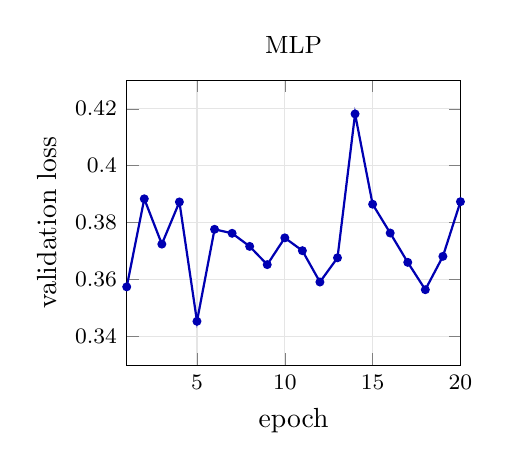
\begin{tikzpicture}
\begin{axis}[
  width=0.48\textwidth, height=5.2cm,
  title={MLP}, title style={font=\small},
  xlabel={epoch}, ylabel={validation loss},
  xmin=1, xmax=20, ymin=0.33, ymax=0.43,
  grid=major, grid style={gray!20}, tick label style={font=\footnotesize}]
\addplot[thick, blue!70!black, mark=*, mark size=1.2pt] coordinates {
(1,0.3575)(2,0.3884)(3,0.3725)(4,0.3873)(5,0.3454)(6,0.3777)(7,0.3763)(8,0.3717)(9,0.3653)(10,0.3747)
(11,0.3702)(12,0.3592)(13,0.3677)(14,0.4182)(15,0.3865)(16,0.3764)(17,0.3661)(18,0.3565)(19,0.3682)(20,0.3874)};
\end{axis}
\end{tikzpicture}\hfill
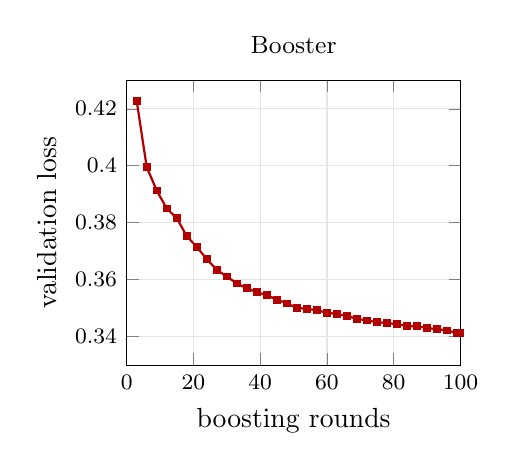
\begin{tikzpicture}
\begin{axis}[
  width=0.48\textwidth, height=5.2cm,
  title={Booster}, title style={font=\small},
  xlabel={boosting rounds}, ylabel={validation loss},
  xmin=0, xmax=100, ymin=0.33, ymax=0.43,
  grid=major, grid style={gray!20}, tick label style={font=\footnotesize}]
\addplot[thick, red!70!black, mark=square*, mark size=1pt] coordinates {
(3,0.4227)(6,0.3995)(9,0.3913)(12,0.385)(15,0.3816)(18,0.3753)(21,0.3715)(24,0.3672)(27,0.3635)(30,0.3611)
(33,0.3587)(36,0.357)(39,0.3556)(42,0.3546)(45,0.353)(48,0.3517)(51,0.3501)(54,0.3498)(57,0.3493)(60,0.3484)
(63,0.348)(66,0.3473)(69,0.3463)(72,0.3457)(75,0.3451)(78,0.3448)(81,0.3444)(84,0.3437)(87,0.3437)(90,0.343)
(93,0.3427)(96,0.3422)(99,0.3413)(100,0.3414)};
\end{axis}
\end{tikzpicture}
\caption{The MLP's validation loss jumps between epochs and was lowest at epoch
$5$, while the booster's falls steadily and was still falling at round $100$
(seed $1$; same vertical scale). In four of five seeds the MLP's best epoch was
among the first five; in all five the booster's best checkpoint was at round
$99$ or $100$.}
\label{fig:adult-curves}
\end{figure}

\Cref{fig:adult-curves} shows why the defaults favour the booster. The MLP,
with a learning rate of $10^{-3}$ and about $815$ steps per epoch, reaches its best
validation loss within a few epochs and then oscillates; keeping the best
checkpoint protects it, but the later epochs add nothing. The booster improves
monotonically and stops because it runs out of rounds, which suggests that more
rounds would widen its lead. The booster's most-used inputs in seed $1$, by
number of splits, were age ($402$), capital gain ($360$), hours per week
($232$), capital loss ($200$) and years of education ($170$).

\section{Limitations}\label{sec:limits}

\begin{description}
  \item[One dataset] The comparison uses one public dataset with default
        settings; it shows how the two models behave out of the box, not which
        is better in general.
  \item[No hyperparameter search] Neither model was tuned. Boosted trees in
        particular usually gain from more rounds and a tuned depth.
  \item[Export gaps] Tree ensembles and CNNs cannot be exported to ONNX yet.
  \item[Small models only] The engine targets models that train in seconds to
        minutes; the CPU default reflects that.
\end{description}

\section*{Preparation}

This paper was drafted with an AI assistant (Claude) from Axon's source code,
README and changelog, and the experiments of \cref{sec:eval} were run for it;
the author is responsible for its content. \Cref{app:provenance} lists the
source of every number.

\section*{License}

\copyright\ 2026 Ryan Wetzstein. This paper is licensed under the Creative
Commons Attribution 4.0 International License (CC BY 4.0,
\url{https://creativecommons.org/licenses/by/4.0/}). The license covers the
text and figures of this paper, not the Axon software, which is licensed under
Apache-2.0.

\begin{thebibliography}{9}
\bibitem{xgboost} T.~Chen and C.~Guestrin. XGBoost: A scalable tree boosting
  system. In \emph{Proceedings of the 22nd ACM SIGKDD International Conference
  on Knowledge Discovery and Data Mining}, pages 785--794, 2016.
\bibitem{abramowitz} M.~Abramowitz and I.~A. Stegun, editors. \emph{Handbook of
  Mathematical Functions}. National Bureau of Standards, 1964.
\bibitem{adult} B.~Becker and R.~Kohavi. Adult. UCI Machine Learning
  Repository, 1996. \url{https://doi.org/10.24432/C5XW20}.
\end{thebibliography}

\appendix
\section{Provenance of numbers}\label{app:provenance}

\begin{table}[htbp]
\centering
\caption{Where each reported number comes from. Source paths are relative to
the \code{axon} repository at commit \code{0991c9c}.}
\label{tab:provenance}
\small
\begin{tabular}{>{\raggedright\arraybackslash}p{0.42\textwidth} >{\raggedright\arraybackslash}p{0.52\textwidth}}
\toprule
Number & Source \\
\midrule
Task rule ($20$ integer classes), $50$ categories, missing tokens & \code{src/tabular.rs}, \code{README.md} \\
Imbalance threshold $3$, weights, unweighted validation loss & \code{src/model.rs}, \code{src/tabular.rs} \\
Weighted cross-entropy normalization & \code{burn-nn} 0.21.0, \code{loss/cross\_entropy.rs} \\
Adam $\beta_1, \beta_2, \epsilon$ & \code{burn-optim} 0.21.0, \code{AdamConfig} defaults \\
CNN layers and defaults & \code{src/model.rs} \\
GPT shape, defaults, initialization, GELU and erf & \code{src/text.rs} \\
Booster defaults, base scores, gradients, leaf value, gain, bins & \code{src/gbdt.rs} \\
Report interval ($40$ reports) & \code{src/model.rs} (\code{GBDT\_REPORTS}) \\
ONNX nodes and opset & \code{src/onnx.rs}; exact match from \code{README.md} \\
Adult class counts, missing rows, input count & computed from the downloaded file; run logs \\
All metrics, curves, best checkpoints, split counts & run logs and confusion matrices of the ten runs \\
Training times & wall-clock time of each run \\
\bottomrule
\end{tabular}
\end{table}

\paragraph{Experiments.} The data is the UCI archive's \code{adult.data},
whose SHA-256 hash begins \code{5b002646}, with a header row added and the
spaces after each comma removed. Axon was built from commit \code{0991c9c}
and reported version 0.11.0. The runs used an Apple A18 Pro CPU (six cores) at
reduced priority, one after another.

\paragraph{Not confirmed.} The ONNX exact-match claim is taken from the
README; the export tests were not re-run. The GPT and CNN were not trained for
this paper. The ten runs are not saved in any repository.

\end{document}
